%% ACM sigconf draft for MARVIN
\documentclass[acmsmall, screen]{acmart}
\usepackage{subcaption}
\usepackage{svg}

\setcopyright{acmlicensed}
\copyrightyear{2025}
\acmYear{2026}
\acmDOI{XXXXXXX.XXXXXXX} % TODO
\acmConference[TEI SDC '26]{TEI Student Design Challenge}{March, 2026}{Chicago, Illinois}
\acmISBN{978-1-4503-XXXX-X/2026/06} % TODO

\AtBeginDocument{\providecommand\BibTeX{{Bib\TeX}}}

\begin{document}

\title{MARVIN: Remote Teleoperation of a Dual-Arm Robot}
\subtitle{Real-time human motion mirroring with client-side ML and ROS2}

%% Authors
\author{Jaeho Cho}
\authornote{Both authors contributed equally to this research.}
\email{jaeho.cho@cooper.edu}
\affiliation{
  \institution{The Cooper Union for the Advancement of Science and Art}
  \city{New York}
  \state{New York}
  \country{USA}
}
\author{Sophia Klymchuk}
\authornotemark[1]
\email{sophia.klymchuk@cooper.edu}
\affiliation{
  \institution{The Cooper Union for the Advancement of Science and Art}
  \city{New York}
  \state{New York}
  \country{USA}
}

\renewcommand{\shortauthors}{Cho and Klymchuk}

\begin{abstract}
MARVIN is a dual-arm teleoperational robot that mirrors a human operator's upper-body motion in real time using just a standard webcam. Client-side MediaPipe models extract 3D pose and hand landmarks, which are transmitted via websocket to a ROS2-MoveIt servoing stack that commands two OpenManipulator-X arms. We detail perception-to-actuation mappings, including geometric formulations for shoulder flexion, shoulder abduction/adduction, and elbow flexion, and describe a web interface that enables intuitive interaction. We report user survey results from local and remote operation, and discuss ethical and societal impacts.
\end{abstract}

%%
%% The code below is generated by the tool at http://dl.acm.org/ccs.cfm.
%%
\begin{CCSXML}
<ccs2012>
   <concept>
       <concept_id>10010583</concept_id>
       <concept_desc>Hardware</concept_desc>
       <concept_significance>500</concept_significance>
       </concept>
 </ccs2012>
\end{CCSXML}

\ccsdesc[500]{Hardware}
%%

\keywords{teleoperation, human-robot interaction, ROS2, MoveIt, MediaPipe}

\received{NA} % TODO
\received[revised]{NA} % TODO
\received[accepted]{NA} % TODO

\maketitle

\section{Introduction}
MARVIN is a teleoperational robot that mirrors the upper-body movements of a human operator in real time. Operation works via a local webcam or a remote connection, where a web application captures the user's webcam stream for pose landmarking, enabling MARVIN to act as a physical avatar across any distance.

MARVIN explores the theme of the 2026 SDC theme of Sensory Rituals through the design of a remotely-operated humanoid robot that reintroduces physicality into digital communication. Contemporarily, much of interpersonal digital interaction occurs via screen-based interfaces that flatten embodied and sensory engagement. Via MARVIN, we seek to restore a sense of physical presence to virtual meetings by allowing its users to inhabit a robot equipped with two controllable arms.

By remotely manipulating the robot via one's own mirrored actions, tangible social connection can be had at-distance, enabling the operator to perform actions, express intentions, and interact with physical environments shared by the receiver.

Furthermore, MARVIN is an accessible platform, as it requires only a standard webcam and Internet interface, which extends this ritual to anyone irrespective of distance, with only minimal technological barriers. This inclusivity broadens the system's use as a tool for fostering shared sensory experiences in remote or hybrid environments. Via its integration of presence, interaction, and accessibility, MARVIN allows tangible rituals to emerge out of traditional confinement and into a process of technological mediation that reconnects individuals to the physical world and to one another.

% \section{Related Work}
% TODO: Add literature comparison and related teleoperation frameworks.

\section{Hardware}
MARVIN uses components from the ROBOTIS OpenManipulator-X platform. Each arm has 5 DOF and is powered by Dynamixel XM430-W350 servos. We utilize two arms attached to an aluminum-beam torso and powered via a Dynamixel U2D2 power hub.

\section{Software}
MARVIN runs on the Humble distribution of ROS2. High-level motion is handled by MoveIt, which translates user commands into low-level commands sent to Dynamixel controllers. A custom URDF/Xacro model encodes simultaneous kinematics, inertial, and control interfaces for both arms.

\subsection{Pose Detection}
OpenCV interfaces a MediaPipe-based pose detector to extract normalized 3D joint landmarks from a webcam stream \cite{noauthor_mediapipe_nodate}. We use shoulder (11,12), elbow (13,14), wrist (15,16), and hip (23,24) landmarks to compute joint angles that are then mapped to MARVIN's kinematic model. Figure \ref{fig:pose-landmarks} displays the landmark labelling scheme.

\subsubsection{Shoulder Flexion}
Let $S$ (shoulder), $E$ (elbow), $H$ (same-side hip), $H_{opp}$ (opposite hip).
\begin{displaymath}
  \mathbf{u}=E-S,\quad \mathbf{v}=H-S,\quad \mathbf{h}=H_{opp}-H,\quad \hat{\mathbf{n}}=\frac{\mathbf{h}}{\lVert\mathbf{h}\rVert}
\end{displaymath}
Project onto the midline plane orthogonal to $\hat{\mathbf{n}}$:
$
\mathbf{u}_\pi=\mathbf{u}-(\mathbf{u}\cdot\hat{\mathbf{n}})\,\hat{\mathbf{n}},\quad
\mathbf{v}_\pi=\mathbf{v}-(\mathbf{v}\cdot\hat{\mathbf{n}})\,\hat{\mathbf{n}}. \\
$
Flexion:
\begin{equation}
\alpha=\arccos \!\left( \frac{\mathbf{u}_\pi \cdot \mathbf{v}_\pi}{\lVert\mathbf{u}_\pi\rVert\, \lVert\mathbf{v}_\pi\rVert} \right)\,.
\end{equation}
Map $\alpha$ to shoulder flexion/extension joint ($J_1$).

\subsubsection{Shoulder Adduction/Abduction}
Let $\mathbf{u}$, $\hat{\mathbf{n}}$ be as above. Project $\mathbf{u}$:
$
\mathbf{u}_\pi=\mathbf{u}-(\mathbf{u}\cdot\hat{\mathbf{n}})\,\hat{\mathbf{n}}.\\
$
Adduction magnitude:
\begin{equation}
\beta=\arccos \!\left( \frac{\mathbf{u}\cdot\mathbf{u}_\pi}{\lVert\mathbf{u}\rVert\, \lVert\mathbf{u}_\pi\rVert} \right)\,.
\end{equation}
Signed ab/adduction can be obtained from $\operatorname{sign}\big((\mathbf{u}\times\mathbf{u}_\pi)\cdot\hat{\mathbf{n}}\big)$. Map to $J_2$.

\subsubsection{Elbow Flexion}
Let $\mathbf{u}$ be as above and forearm $\mathbf{f}=E-W$. Then
\begin{equation}
\theta=\arccos \!\left( \frac{\mathbf{u}\cdot\mathbf{f}}{\lVert\mathbf{u}\rVert\, \lVert\mathbf{f}\rVert} \right)\,.
\end{equation}
Map $\theta$ to elbow joint $J_3$.

\subsubsection{Hand Open/Close}
Using the Hand Landmarker (labels shown in Figure \ref{fig:hand-landmarks}), define a reference length from wrist (0) to middle-finger MCP (9). We mark a hand as open if fewer than three fingertips among indices \{4,8,12,16,20\} lie closer to the wrist than the reference. We then publish binary open/closed messages to drive the gripper.

\begin{figure}[htbp]
  \centering
  \begin{subfigure}[b]{0.45\linewidth}
    \centering
    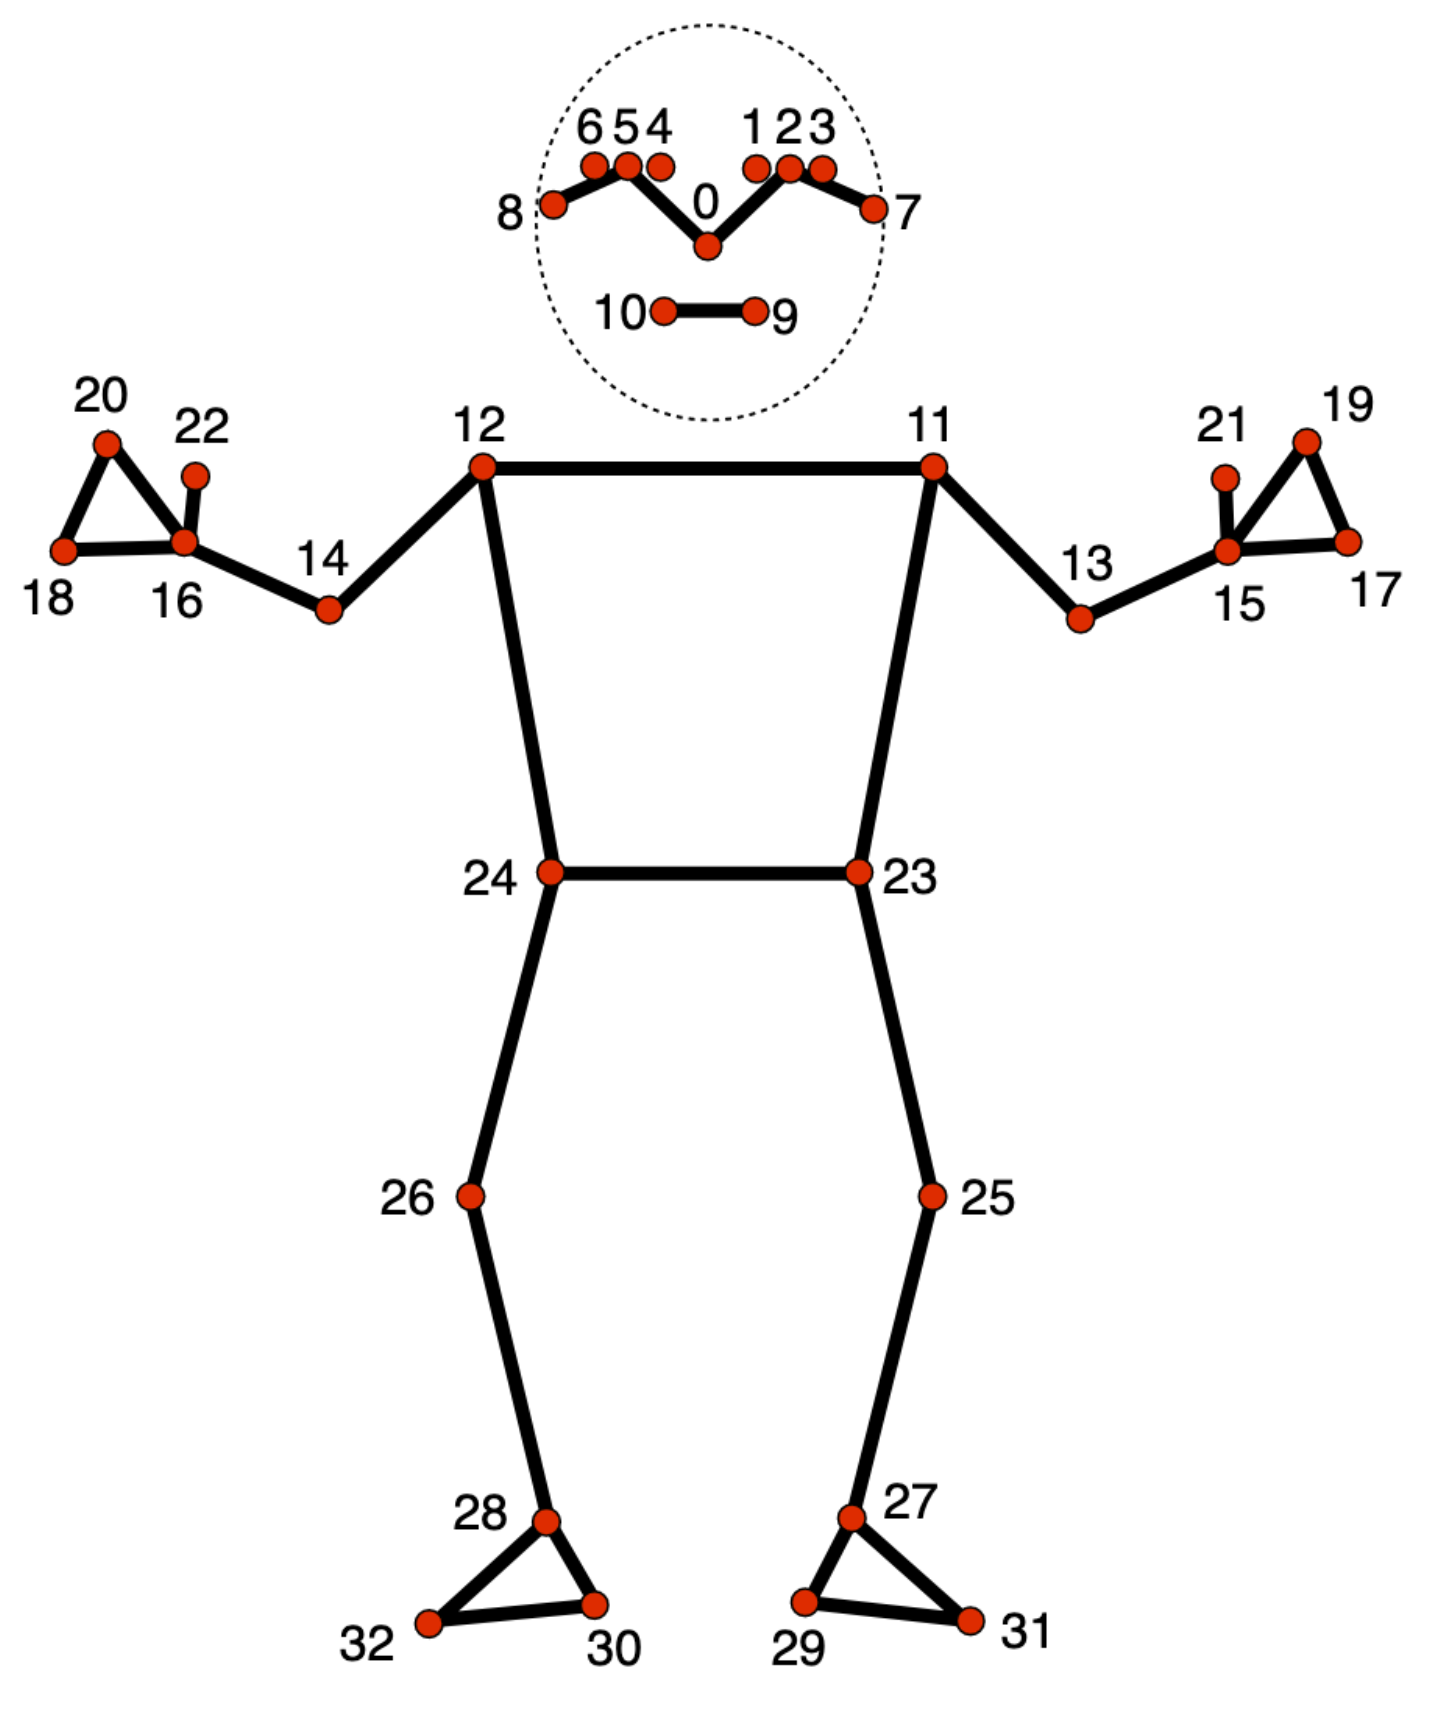
\includegraphics[width=\linewidth]{assets/pose-landmarks.png}
    \caption{MediaPipe Pose Landmarks. The pose landmarker model tracks 33 body landmark locations, representing the approximate location of the labeled body parts.}
    \Description{A diagram of a human figure with 33 labeled landmarks, including shoulders, elbows, wrists, hips, knees, and ankles.}
    \label{fig:pose-landmarks}
  \end{subfigure}
  \hfill
  \begin{subfigure}[b]{0.45\linewidth}
    \centering
    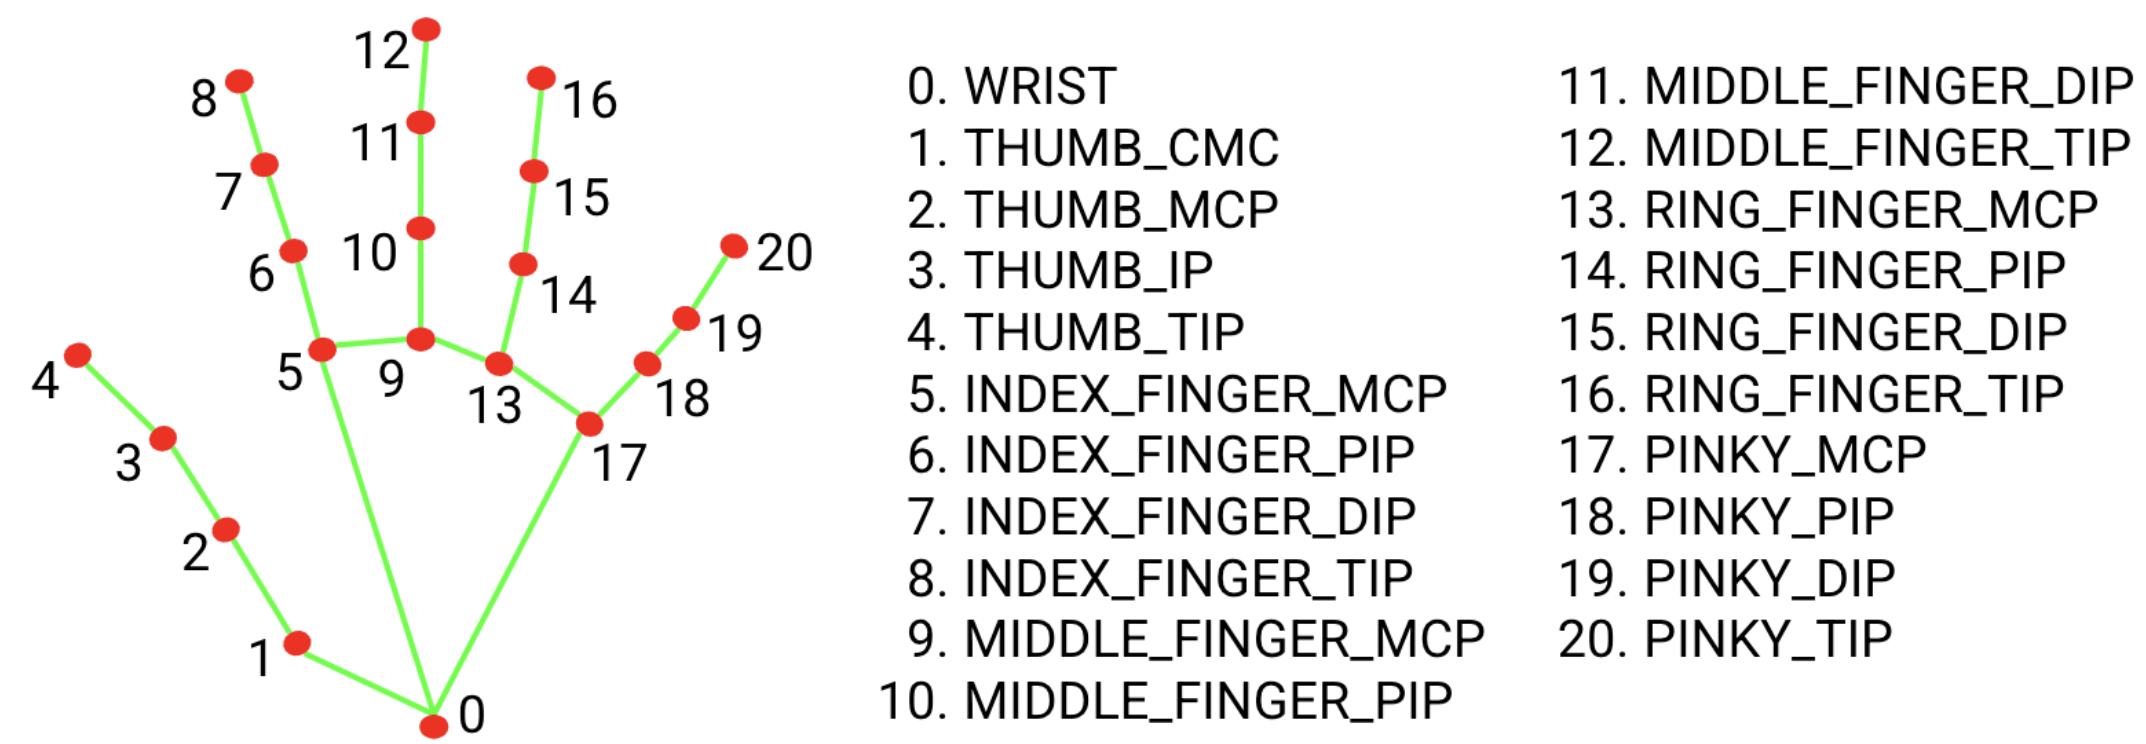
\includegraphics[width=\linewidth]{assets/hand-landmarks.png}
    \caption{MediaPipe Hand Landmarks. The hand landmark model bundle detects the keypoint localization of 21 hand-knuckle coordinates within the detected hand regions.}
    \Description{A diagram of a hand with 21 labeled landmarks, including wrist, palm, and finger joints.}
    \label{fig:hand-landmarks}
  \end{subfigure}
  \caption{Comparison of MediaPipe landmark models: (A) Pose and (B) Hand.}
  \label{fig:landmarks-comparison}
\end{figure}

\subsection{Control}
We use MoveIt real-time servoing with two independent kinematic chains, one per arm. Each chain is associated with a servoing node that subscribes to desired joint velocities. These velocities are computed from the error between detected target joint angles and current joint states from the \texttt{/joint\_states} topic, before being scaled by gains and sent as \texttt{JointJog} commands. Figure \ref{fig:rosgraph} shows the ROS2 node and topic architecture.

\begin{figure}[htbp]
  \centering
  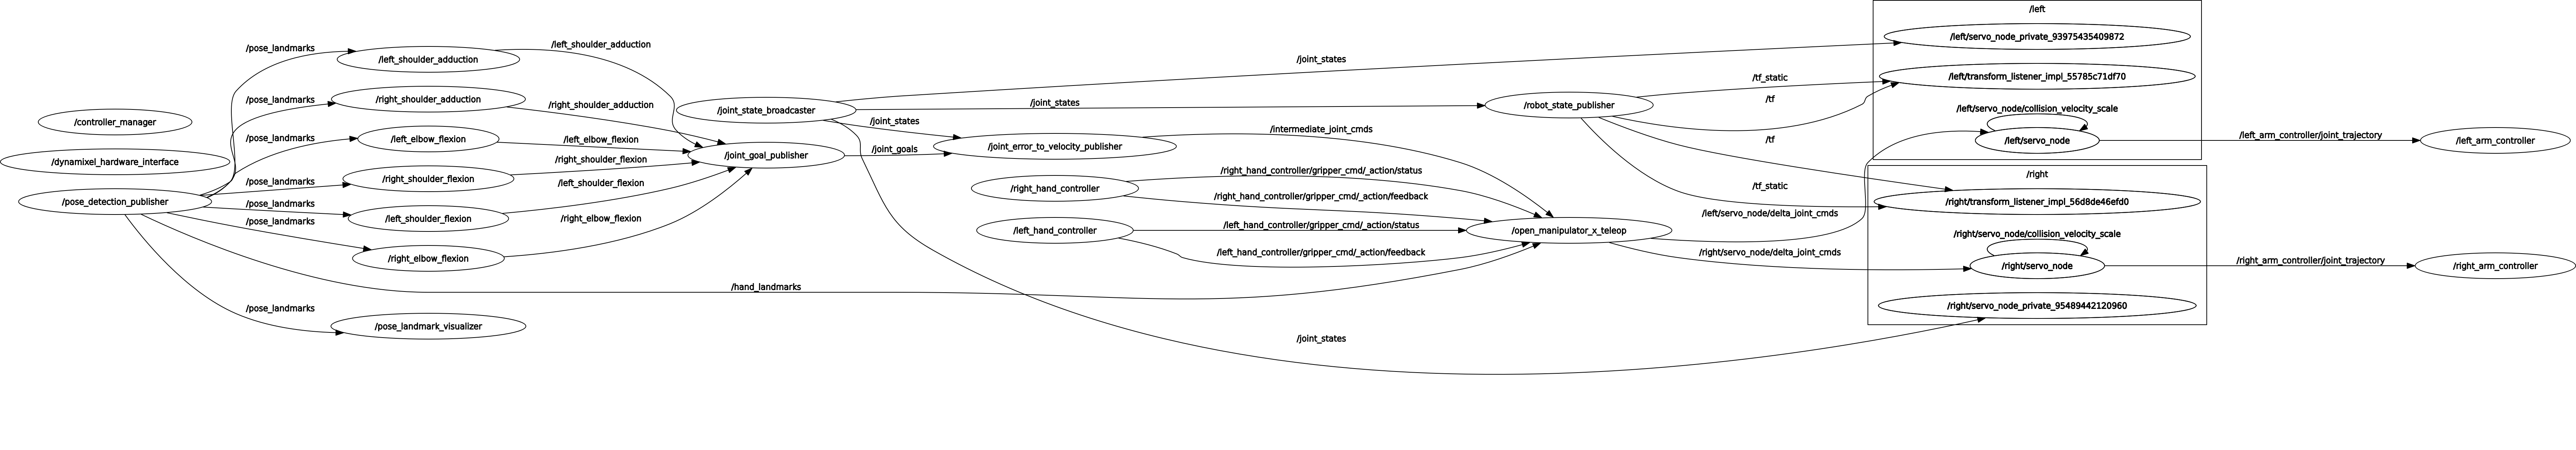
\includegraphics[width=\linewidth]{assets/rosgraph}
  \caption{ROS rqt graph: nodes circled and topics labeled on connections between nodes.}
  \Description{ROS2 rqt graph displaying nodes and topics}
  \label{fig:rosgraph}
\end{figure}

\section{Website}
The website functions as the browser-based front end of MARVIN’s remote teleoperation system. It captures the user’s webcam stream, performs local pose and hand landmark inference, and transmits the previously mentioned key pose landmarks directly to MARVIN, while the hand landmarks are processed locally asforementioned and the boolean status of each hand is then sent to MARVIN. The website also embeds a live video stream of the robot, allowing visual feedback during operation. 

Implemented entirely in client-side JavaScript using the MediaPipe Tasks API, the system requires no native installation or external dependencies. Figure \ref{fig:web} shows a screenshot of the web interface. A compact control panel enables users to start or stop the camera, select inference model complexity, and toggle streaming to the ROSBridge server, which exposes \texttt{pose\_landmarks} and \texttt{hand\_landmarks} topics for downstream motion control.

\begin{figure}[htbp]
  \centering
  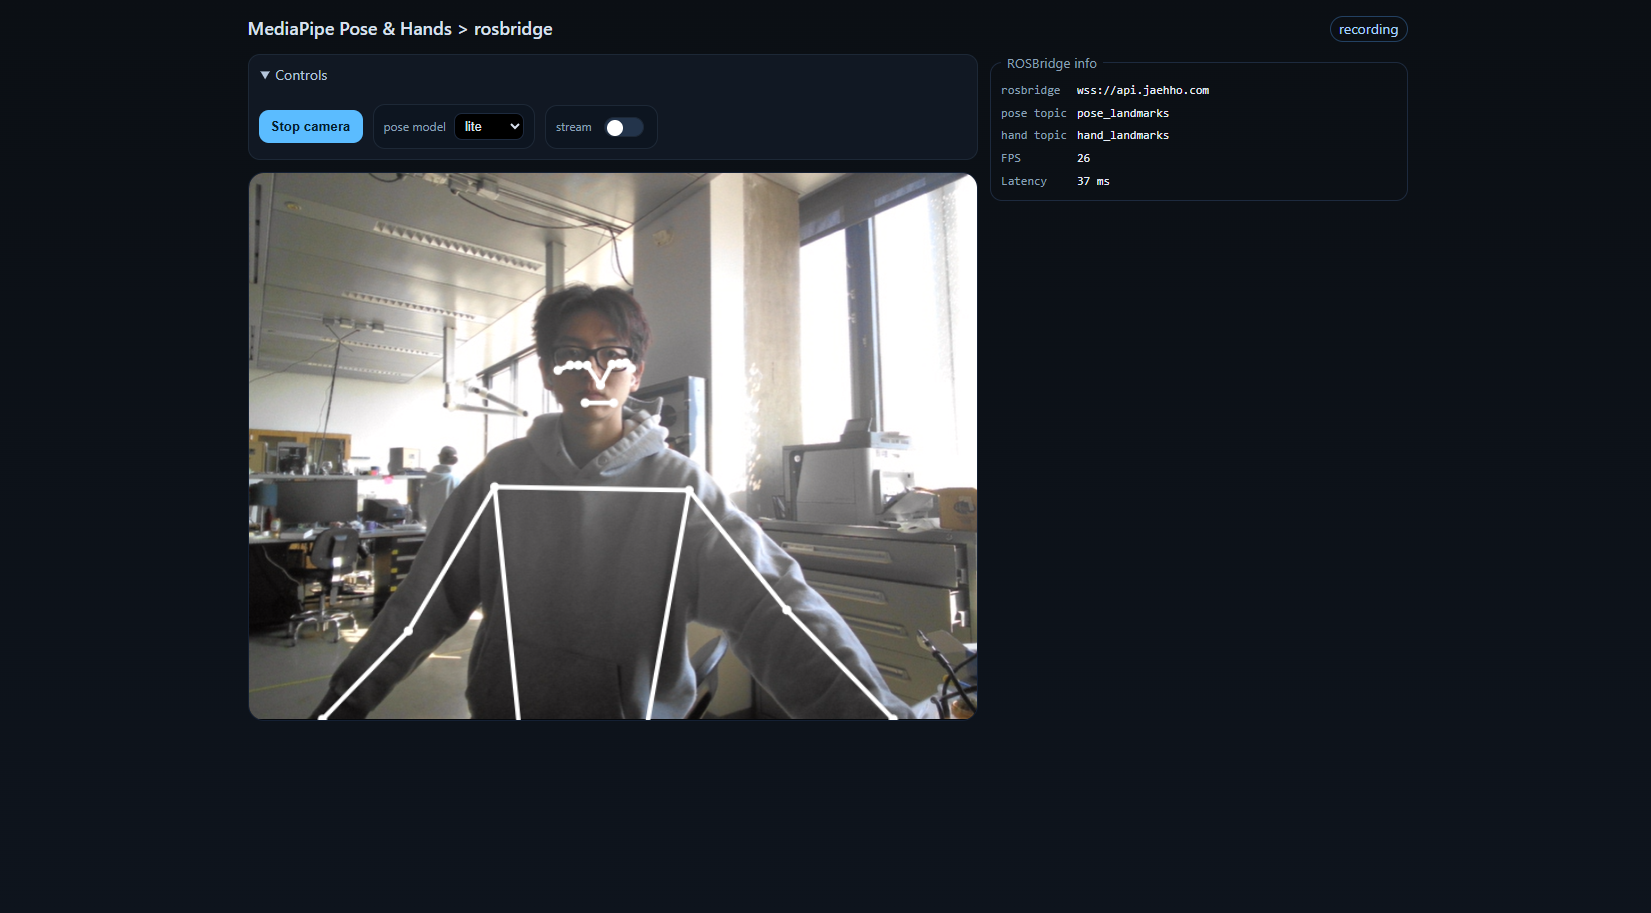
\includegraphics[width=\linewidth]{assets/web}
  \caption{Screenshot of MARVIN website: livestream of MARVIN in center, webcam feed and landmark overlay on right. Connection information below MARVIN livestream and controls below webcam feed.}
  \Description{A screenshot of the web interface showing video feed, control buttons, and status indicators.}
  \label{fig:web}
\end{figure}

The connection to MARVIN is made via ROSBridge over WebSocket, allowing seamless communication between the browser and the ROS2 backend. Figure \ref{fig:pipeline} illustrates the communication pipeline from user to MARVIN.

\begin{figure}[htbp]
  \centering
  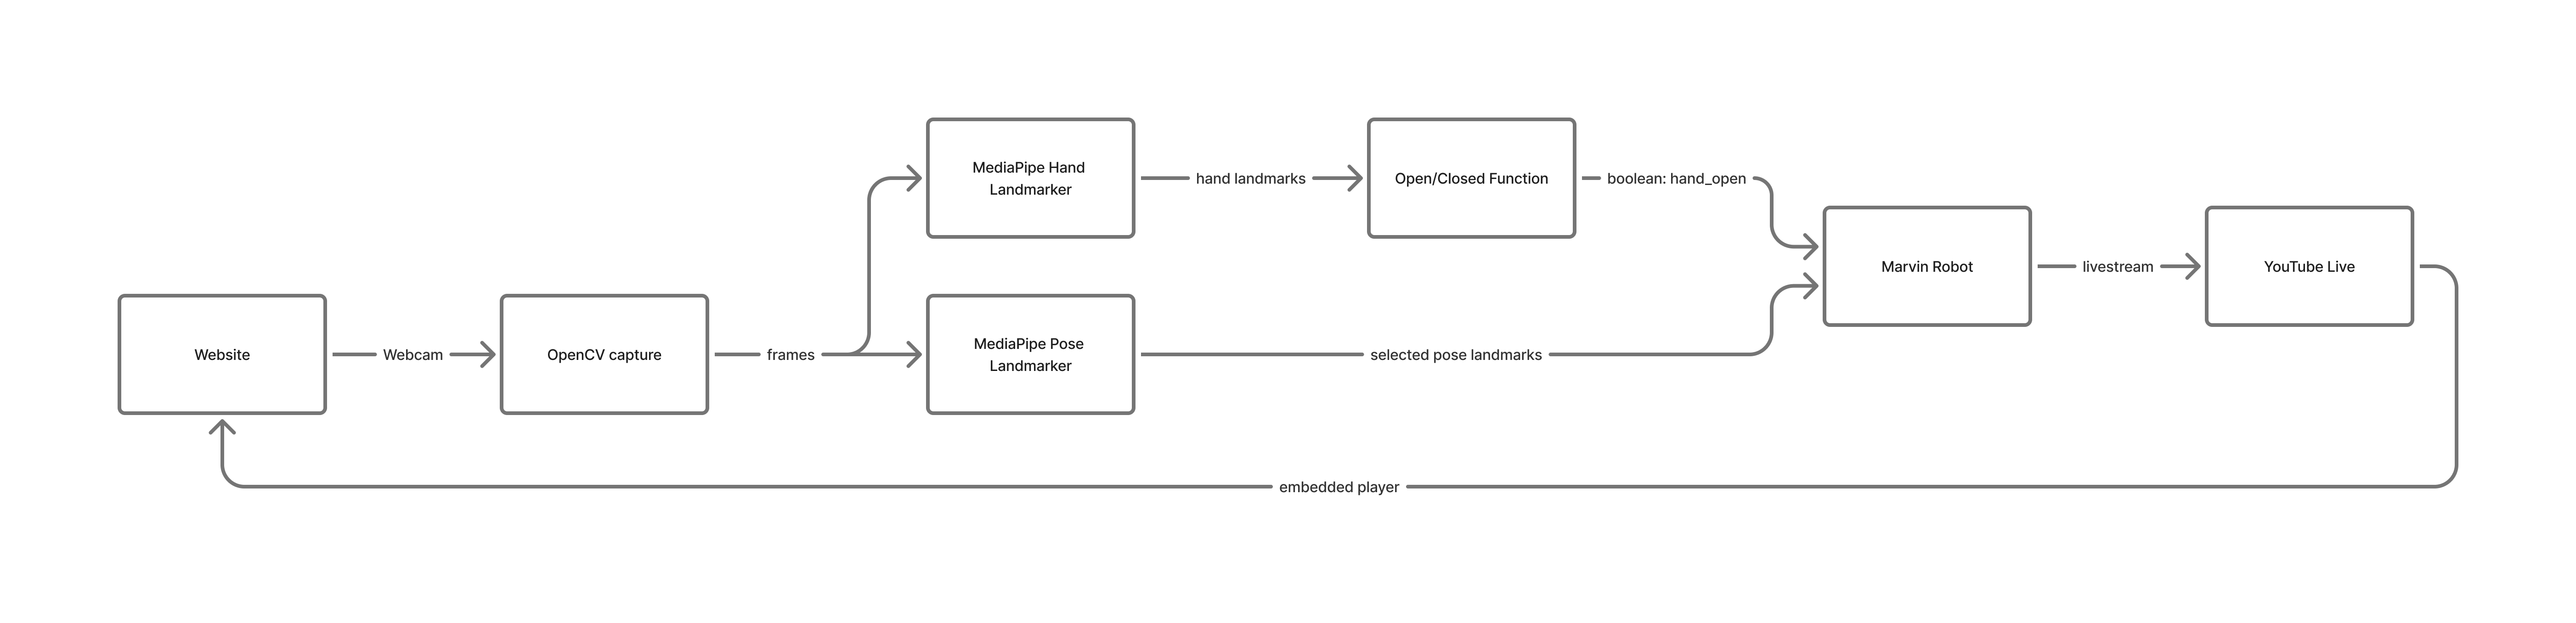
\includegraphics[width=\linewidth]{assets/MARVIN Communication Pipeline}
  \caption{Communication pipeline from user to MARVIN.}
  \Description{Diagram of communication pipeline}
  \label{fig:pipeline}
\end{figure}

\begin{figure}[htbp]
  \centering
  \includegraphics[width=0.5\linewidth]{assets/marvin}
  \caption{MARVIN}
  \Description{Photograph of MARVIN}
  \label{fig:photo}
\end{figure}

\section{Operation and User Study}
MARVIN was tested in local operation during the Cooper Union End of Year Show of May 2025. The robot mirrored onlooker movements in real time, and we received qualitative feedback requesting the addition of hand gestures for a more natural feeling. This informed subsequent implementation of the hand landmark module and gripper control. 

We additionally tested remote operation of MARVIN with peer volunteers from the Cooper Union community, while the robot was stationed in the lab. Participants were interacted with the website and controlled MARVIN from a separate room. Despite attempts to optimize low latency communication, there is a noticeable lag between operator movement and live stream video feedback, with an average round-trip time of \textit{~3} s. The delay includes the the websocket transmission time, processinng time on the ROS2 side, and return youtube streaming lag.

\section{Safety and Limits}
With a previous incident of MARVIN damaging itself during testing, we implemented several safety measures. We enforce velocity, position, and current limits at the controller, while the MoveIt servo planning predicts and prevents self-collisions.

\section{Discussion}
MARVIN demonstrates that fully client-side inference is viable for dual-arm mirroring. Remaining gaps include wrist pronation supination estimation, depth ambiguity in monocular input, and gripper force control. Future work includes (1) integrating depth perception, (2) incorporating joint configurations and kinematic structures more closely aligned with human anatomy, (3) self-calibration, and (4) extending to mobile bases for extended telepresence.

\section{Ethical and Societal Impact}
Telepresence expands access but raises safety and privacy concerns. We transmit only necessary landmark data, that does not include any identifying user information, including the webcam feed.

\section{Conclusion}
We provided a remote teleoperation system that minimizes user setup while retaining intuitive, low-latency control of a dual-arm robot. All code and hardware designs are open-sourced at \url{https://github.com/jaehho/marvin}.

\begin{acks}
We thank The Cooper Union community for volunteering and supporting facilities.
\end{acks}

\bibliographystyle{ACM-Reference-Format}
\bibliography{references}

\end{document}
